% --- INIZIO slide1_gap_analysis.tex ---
\begin{frame}{Gap Analysis: The "Deformability-Energy Dilemma"}
    \begin{columns}
        % Colonna Testo (Sinistra)
 \begin{column}{0.55\textwidth}
            \begin{itemize}
                \item \textbf{The Current Compromise}
                \begin{itemize}
                    \item \textit{SACH:} good cushioning, but high energy dissipation.
                    \item \textit{ESR (Carbon Fiber):} excellent return but fixed stiffness (harmful load transfer).
                \end{itemize}
                
                \vspace{0.4cm}
                
                \item \textbf{The Real Technological Gap:}
                \begin{itemize}
                    \item Lack of a \textbf{100\% passive} solution (no electronics) that is \textbf{dynamically adaptive}.
                \end{itemize}
                
                \vspace{0.4cm}
                
                \item \textbf{The Necessity:} 
                \begin{itemize}
                    \item Moving beyond the linearity of traditional materials to overcome mechanical limits.
                \end{itemize}
            \end{itemize}
        \end{column}
        
        % Colonna Immagine (Destra)
        \begin{column}{0.45\textwidth}
            \centering
            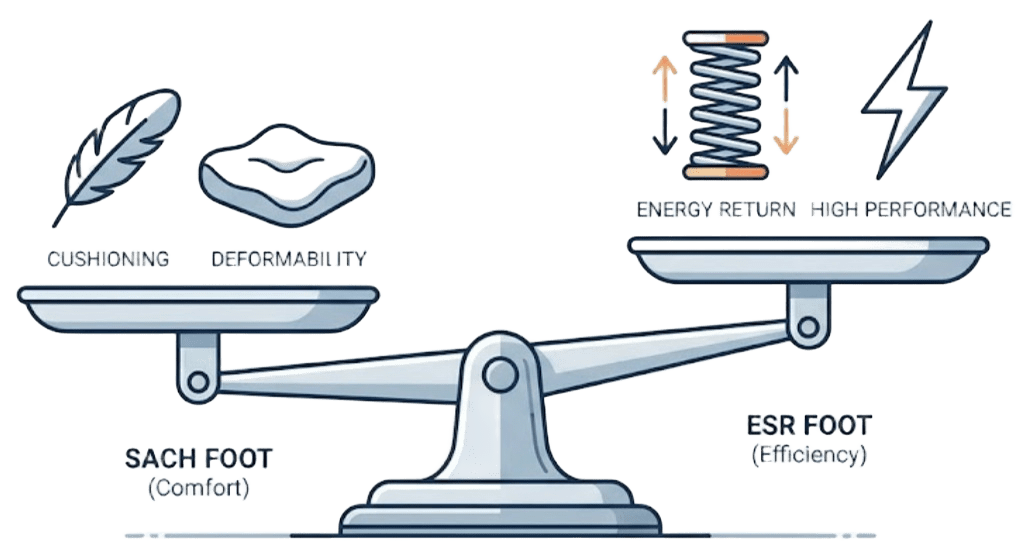
\includegraphics[width=1.0\textwidth]{image/bilancia.png}
        \end{column}
    \end{columns}
\end{frame}